\documentclass[10pt]{beamer}
%
% Choose how your presentation looks.
%
% For more themes, color themes and font themes, see:
% http://deic.uab.es/~iblanes/beamer_gallery/index_by_theme.html
%
\mode<presentation>
{%
  \usetheme{metropolis}      % or try Darmstadt, Madrid, Warsaw, ...
  \usecolortheme{rose} % or try albatross, beaver, crane, ...
  \usefonttheme[onlymath]{serif}
  \setbeamertemplate{navigation symbols}{}
  \setbeamertemplate{caption}[numbered]
} 

\usepackage[english]{babel}
\usepackage[utf8x]{inputenc}
\usepackage[linesnumbered,ruled]{algorithm2e}
\usepackage{amsmath, amssymb}
\usepackage{amsthm}
\usepackage{subcaption}
\usepackage{listings}

%tikz packages
\usepackage{tikz}
\usetikzlibrary{trees,er,matrix,mindmap,backgrounds}
\usetikzlibrary{shadings,intersections,calc}
\usetikzlibrary{shapes,arrows,patterns,snakes}
\usetikzlibrary{automata,shadows,fit,fadings,matrix,positioning,trees}
\usepackage{pgfplots}
\usepackage{pgfkeys}
\usepackage{mathrsfs}
\usepackage{multirow}
\usepackage{booktabs}
\usepgfplotslibrary{units}
\pgfdeclarelayer{nodelayer}
\pgfdeclarelayer{edgelayer}
\pgfsetlayers{edgelayer,nodelayer,main}

\title[Combined Proof Methods for \system{K}{n}{}]{\large Combined Proof Methods for Multimodal Logic}
\author{Daniella Angelos}
\institute{Cl\'audia Nalon --- University of Brasilia}
\date{March 20, 2018}

\newcommand{\ksp}{K\kern -.1em \raisebox{-.24em}{S}\kern -.05em P\xspace}
\newcommand{\then}{\Rightarrow}
\renewcommand{\iff}{\Leftrightarrow}


\newcommand{\agent}{\ensuremath{a}}
\newcommand{\Agents}{\ensuremath{{\mathcal{A}}}}
\newcommand{\Prop}{\ensuremath{{\mathcal{P}}}}
\newcommand{\wff}{\WFF{\system{K}{n}{}}{}}
\newcommand{\wffml}{\ifmmode\text{WFF}^{\scriptsize ml}_{\scriptsize \system{K}{n}{}}}
\newcommand{\sat}[3]{\ensuremath{\langle #1, #2 \rangle \models #3}}
\newcommand{\Model}{\ensuremath{\mathcal{M}}}
\newcommand{\formula}{\ensuremath{\varphi}}
\newcommand{\trule}{\ensuremath{\sigma}}
\newcommand{\calculus}[1]{\ensuremath{\mathcal{C}_{#1}}}
\newcommand{\Literals}{\ensuremath{\mathcal{L}}}
\newcommand{\ml}{\ensuremath{i}}
\newcommand{\cprop}[2]{\ensuremath{\ml: \bigvee^{#1}_{#2 = 1}l_{#2}}}
\newcommand{\cneg}{\ensuremath{\ml: l \then \pos{a}m}}
\newcommand{\cpos}{\ensuremath{\ml: l \then \nec{a}m}}
\renewcommand{\stackrel}[1]{\ensuremath{\overset{\text{#1}}{=}}}
\newcommand{\ckn}{\ensuremath{\cal{C}_{\system{K}{n}{}}}}
\newcommand{\ex}{\ensuremath{\nec{}(p \then \pos{})}}
\newcommand{\clause}{\ensuremath{\omega}}
\newcommand{\passignment}{\ensuremath{\rho}}
\newcommand{\res}{\ensuremath{\odot}}

\newtheorem{theorem}{Theorem}[section]
\newtheorem{lemma}[theorem]{Lemma}
%\newtheorem{example}[subsection]{Example}
%\newtheorem{proposition}[theorem]{Proposition}
%\newtheorem{corollary}[theorem]{Corollary}
%\newtheorem{definition}[theorem]{Definition}

%\newenvironment{proof}[1][Proof]{\begin{trivlist}
%\item[\hskip \labelsep {\bfseries #1}]}{\end{trivlist}}
%\newenvironment{example}[1][Example]{\begin{trivlist}
%\item[\hskip \labelsep {\bfseries #1}]}{\end{trivlist}}
%\newenvironment{remark}[1][Remark]{\begin{trivlist}
%\item[\hskip \labelsep {\bfseries #1}]}{\end{trivlist}}

\newcounter{example}
\newenvironment{example}[1][]{\refstepcounter{example}\par\medskip
   \noindent \textbf{Example~\theexample #1.} \rmfamily}{\medskip}


\ifx\fmtname\@psfmtname \else \def\cmsy@{2}\fi % make sure we get cmsy
\def\sometime{\mathord{\hbox{\normalsize$\mathchar"0\cmsy@7D$}}}


\newcommand{\always}{\raisebox{-.2ex}{
           \mbox{\unitlength=0.9ex
           \begin{picture}(2.3,2.3)
           \linethickness{0.06ex}
           \put(0,0){\line(1,0){2.3}}
           \put(0,2.3){\line(1,0){2.3}}
           \put(0,0){\line(0,1){2.3}}
           \put(2.3,0){\line(0,1){2.3}}
           \end{picture}}}
          \,}

\newcommand{\alwaysi}[1]{\raisebox{-.2ex}{
           \mbox{\unitlength=0.9ex
           \begin{picture}(2,2)
			   \linethickness{0.06ex}
			   \put(0,0){\line(1,0){2}}
			   \put(0,2){\line(1,0){2}}
			   \put(0,0){\line(0,1){2}}
			   \put(2,0){\line(0,1){2}}
                           \put(0.5,0.5){\scriptsize$#1$}
			   \end{picture}}}}

\newcommand{\nec}[1]{\!\alwaysi{#1}\,}
\newcommand{\pos}[1]{{	   \mbox{\unitlength=0.8ex
			   \begin{picture}(2,2)
			   \linethickness{0.06ex}
			   \put(0,0){$\sometime$}
                           \put(0.6,0.4){\tiny$#1$}
			   \end{picture}}}\,}

%\newcommand{\nec}[1]{{	   \mbox{\unitlength=1.5ex
			   %\begin{picture}(2,2)
			   %\linethickness{0.06ex}
			   %\put(0,0){$\always$}
                           %\put(0.8,0.4){\footnotesize$ #1$}
			   %\end{picture}}}\,}

%\newcommand{\pos}[1]{{	   \mbox{\unitlength=1.5ex
			   %\begin{picture}(1.5,1.5)
			   %\linethickness{0.06ex}
			   %\put(0,0){$\sometime$}
                           %\put(0.6,0.4){\footnotesize$#1$}
			   %\end{picture}}}\,}

%\newcommand{\pos}[1]{\sometime _{#1}}
\newcommand{\onlyif}{\Leftarrow}
\newcommand{\ifonlyif}{\Leftrightarrow}
\newcommand{\tvalue}[1]{\mbox{\it #1\/}}
\newcommand{\constant}[1]{\mbox{\rm\bf #1}}
\newcommand{\system}[3]{\raisebox{.2ex}[1.2ex]{\raisebox{-.2ex}{{\sf #1}}{$_{#2}^{#3}$}}}
%\newcommand{\system}[3]{{\sf #1}$_{#2}^{#3}$}
\newcommand{\set}[1]{\mbox{$\mathcal{#1}$}}
\newcommand{\WFF}[2]{{\sf WFF}{\mbox{$_{\mbox{\small\sf #1}^{#2}}$}}}
\newcommand{\know}[1]{\mbox{K$_{#1}\,$}}
\newcommand{\knownot}[1]{\mbox{$\nec{#1}\neg\,$}}
\newcommand{\believe}[1]{\mbox{B$_{#1}\,$}}
\newcommand{\relation}[2]{\mbox{$\mathcal #1$$_{#2}$}}
%\newcommand{\universal}{\always^{*}}
\newcommand{\universal}{\always^*}
\newcommand{\snf}[1]{{\sf SNF}\mbox{$_{\mbox{\scriptsize #1}}$}}
\newcommand{\binomial}[2]{\left(\! \begin{array}{c}
                                 #1\\
                                 #2
                                 \end{array}
                          \!\right )}
\newcommand{\ap}[1]{\alpha(#1)}

\newcommand{\ib}{\bf}

\newcommand{\NKN}{\hbox{\it NKN}}
\newcommand{\NEW}{\hbox{\it NEW}}


\newcommand{\Nat}{\mbox{$\mathbb N$}}

%\newcommand{\comment}[1]{}
     
\newcommand{\cfalse}{\constant{false}}
\newcommand{\ctrue}{\constant{true}}
\newcommand{\st}{\ensuremath{w}}
\newcommand{\St}{\ensuremath{W}}
\newcommand{\depth}{\sf profundidade}
\newcommand{\model}[1]{{\cal #1}}

\begin{document}

\begin{frame}
  \titlepage
\end{frame}

% Uncomment these lines for an automatically generated outline.
%\begin{frame}{Outline}
%  \tableofcontents
%\end{frame}

\section{Introduction}

\begin{frame}{Logic}
    \begin{block}{in Computer Science:}
        Develop languages to model situations
    \end{block}
\end{frame}

%\begin{frame}{Languages}
%\end{frame}

\begin{frame}
    \frametitle{Languages}   
    \begin{center}
        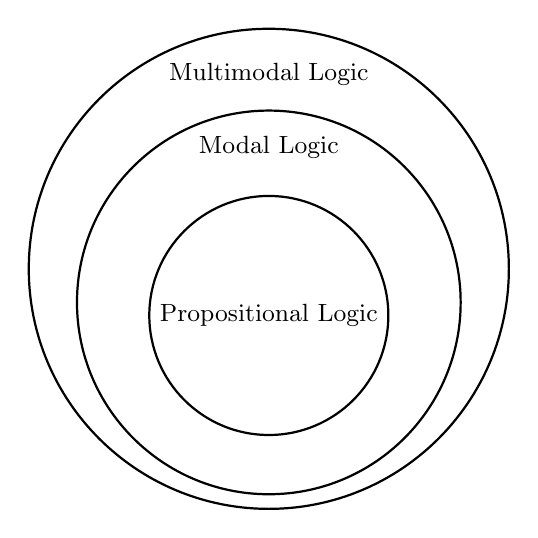
\begin{tikzpicture}[->,circle,draw,node distance=3cm]
            \node[circle,draw,thick,minimum width=2cm,text depth =
            5cm](w0){\small Multimodal Logic};
            \node[circle,draw,thick,minimum width=1.5cm,text depth =
            4cm](w1) at ([yshift=7.5em]w0.south) {\small Modal Logic};
            \node[circle,draw,thick,minimum width=0.3cm](w2) at
            ([yshift=6.5em]w1.south) {\small Propositional Logic};
            %\path[thick] (w0) edge [above] node {1} (w1)
            %(w1) edge [above,loop] node {2} (w1)
            %(w1) edge [above] node {2} (w2)
            %(w0) edge [above] node {1} (w3);
        \end{tikzpicture} 
    \end{center}
\end{frame}

\begin{frame}
    \frametitle{Multimodal Logic (\system{K}{n}{})}
        \begin{itemize}
            \item Propositional Symbols $(\mathcal{P} = \{p, q, r \ldots\})$
            \item Operators $(\neg,\lor, {\color{red} \nec{a}})$
                with ${\color{red}\agent \in \Agents =
                \{1,\ldots,n\}}$
    \end{itemize}
\end{frame}

\begin{frame}{Multimodal Logic (\system{K}{n}{})}
    \begin{block}{Well Formed Formulae (WFF)}
            \begin{itemize}
                \item Propositional Symbols $\cal{P}$
                \item If $\varphi$ and $\psi$ are each a WFF then also are:
                    \begin{enumerate}%[<+- | visible@+(1)->]
                        \item $\neg \formula$
                        \item $\formula \lor \psi$
                        \item $\nec{a} \formula$
                    \end{enumerate}
            \end{itemize}
        \end{block}
\end{frame}

\begin{frame}{Semantics}
    Let $W$ be a set of possible worlds and $R_a$ a binary relation over these
    worlds for some $\agent \in \Agents$:

  \begin{itemize}
      \visible<1->{\item[] {\color{red}Possibility:} $\pos{a} \formula$ is true
              at $\st \in W$ iff \formula~is true at
          some $\st' \in W$ such that $\st R_a \st'$}
      \visible<2->{\item[] {\color{red}Necessity:} $\nec{a} \formula$ is true
              at $\st \in W$ iff \formula~is true at
          all $\st' \in W$ such that $\st R_a \st'$}
  \end{itemize}
\end{frame}

\begin{frame}
    \frametitle{Example}
    \begin{columns}[T] % align columns
        \begin{column}{.63\textwidth}
            \begin{center}
                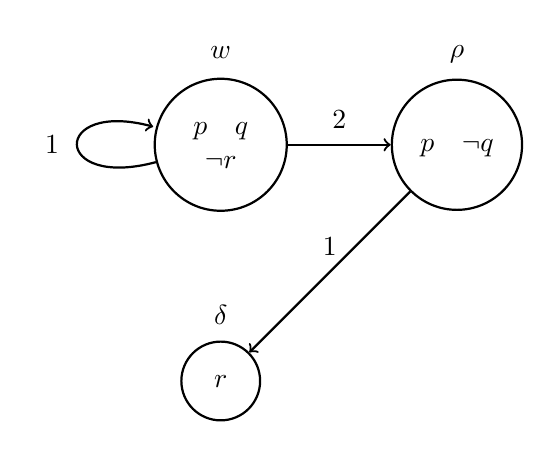
\begin{tikzpicture}[->,circle,draw,node distance=3cm]
                    \node[circle,draw,thick,label=90:$\st$](w0){$
                        \begin{array}{c}
                            p \quad q\\
                            \neg r
                        \end{array}
                    $};
                    \node[circle,draw,thick, label=90:$\rho$,right of=w0](w1){$
                        \begin{array}{c}
                            p \quad \neg q
                        \end{array}
                    $};
                    \node[circle,draw,thick, label=90:$\delta$,below of=w0](w2){$
                        \begin{array}{c}
                            r
                        \end{array}
                    $};
                    \path[thick] (w0) edge [above,loop left] node {1} (w0)
                    %(w1) edge [above,loop right] node {2} (w1)
                    (w0) edge [->,above] node {2} (w1)
                    (w1) edge [->,above] node {1} (w2);
                \end{tikzpicture}
            \end{center}
        \end{column}%
        \hfill%
        \visible<2->{\
            \begin{column}{.48\textwidth}
                Formulae true in $\st$:
                \begin{itemize}
                    \item[] $\nec{1} p$ \onslide<3->{: modal level of $p$ = 1}
                    \item[] $\nec{1} q \wedge \nec{2} \neg q$
                    \item[]  $\pos{2} \pos{1} r$ \onslide<4->{: modal level of
                        $r$ = 2}
                \end{itemize}
            \end{column}%
        }
    \end{columns}
\end{frame}

\begin{frame}
    \frametitle{Model - Kripke Structure} 
    \begin{center}
        {\Large
            $\Model = (W,\st_0,R_1, \ldots, R_n, \pi )$
        }
    \end{center}

    \begin{itemize}[<+- | visible@+(1)->]
       \item Set of possible worlds $W$
       \item Root of model $\st_0 \in W$
       \item A finite number of binary relations $R_a$ over the worlds in $W$,
           $R_a \subseteq W \times W$, with $\agent \in \Agents$
       \item Valuation function to propositional symbols $\pi : W \times \mathcal{P}
           \rightarrow \{true, false\}$
   \end{itemize} 
\end{frame}

\begin{frame}{Satisfiability Relation}
    Let \formula~be a WFF and \tuple~a model in \system{K}{n}{}:

    \visible<2->{\sat{\Model}{\st}{\formula}}
    \begin{itemize}[<+- | visible@+(2)->]
        \item \sat{\Model}{\st}{p} iff $\pi(\st, p) = true$
        \item \sat{\Model}{\st}{\neg \psi} iff $\langle \Model , \st \rangle
            \not \models \psi$
        \item \sat{\Model}{\st}{\psi \lor \delta} iff \sat{\Model}{\st}{\psi} or
            \sat{\Model}{\st}{\delta}
        \item \sat{\Model}{\st}{\nec{a} \psi} iff for all $\st' \in W$ such that
        $\st R_a \st'$, with $\agent \in \Agents$, we have that
    \sat{\Model}{\st'}{\psi}
    \end{itemize}
    
\end{frame}

\begin{frame}{Satisfiability}
    A formula $\formula \in $ WFF is said to be \emph{locally satisfiable} in
    \system{K}{n}{} if exists a model \Model~such that
    \sat{\Model}{\st_0}{\formula}.

    \visible<2->{{\color{red}$\Model \models_L \formula$}}

    \vspace{0.6cm}
    \visible<3->{A formula $\formula \in $ WFF is said to be \emph{globally
    satisfiable} in \system{K}{n}{} if exists a model \Model~such that
    \sat{\Model}{\st}{\formula} for all $\st$.}

    \visible<4->{{\color{red}$\Model \models_G \formula$}}

    \vspace{0.6cm}
    \visible<5->{A set $\Formulae$ of WFF is said to be (locally of globally)
    satisfiable, if the conjunction of each $\formula \in \Formulae$ is
    satisfiable.}
\end{frame}

\begin{frame}{Problem}
    Given any set $\Phi$ of well formed formulae, to determine if $\Phi$ is
    (locally or globally) satisfiable in \system{K}{n}{}.

    \begin{itemize}[<+- | visible@+(1)->]
        \item Local satisfiability: PSPACE-Complete (Halpern and Moses -- 1992),
        \item Global satisfiability: EXPTIME-Complete (E. Spaan -- 1993).
    \end{itemize} 
    
\end{frame}

\section{Layered Resolution}
\begin{frame}
    \frametitle{Clauses in \snf{\system{K}{n}{}}} 
    {\Large
        \begin{center}
        \begin{equation*} \bigwedge_i ml: C_i \end{equation*}
        \end{center}
    }
    \begin{itemize} 
        \onslide<2->{\item literal clause:
        \begin{center} $ml: \bigvee^r_{b=1} l_b$ \end{center}}
        \onslide<3->{\item $\agent$-positive clause:
        \begin{center} $ml: l' \Rightarrow \nec{\agent} l$ \end{center}}
        \onslide<4->{\item $\agent$-negative clause:
        \begin{center} $ml: l' \Rightarrow \pos{\agent} l$ \end{center}}
    \end{itemize} 
    \visible<5->{where $l$ is a propositional symbol or its negation}

\end{frame}

\begin{frame}{Calculus}
\begin{center}
$
\begin{array}{lrl}
\mbox{[LRES]} &ml: & D \lor l\\
 &ml: & D' \lor \neg l\\  \cline{2-3}
    &ml: & D \lor D'
\end{array}
$
\end{center}
\end{frame}

\begin{frame}{Calculus}
    \scriptsize
\begin{minipage}[t]{0.48\linewidth}
    $
    \begin{array}{lrl}
        \mbox{[GEN1]} & ml: & {l'}_1  \then  \nec{a}\neg l_1 \\
                  & \qquad \vdots  \\
                  & ml: & {l'}_m  \then  \nec{a}\neg l_m \\
                  & ml: & l'  \then  \pos{a}\neg  l \\
                  & ml + 1:  & l_1 \lor \ldots \lor l_m \lor l \\  \cline{2-3}
                  & ml:  & \neg {l'}_1 \lor \ldots \lor \neg {l'}_m \lor \neg l'
    \end{array} 
    $
\end{minipage}\hfill
\begin{minipage}[t]{0.48\linewidth}
    $
    \begin{array}{lrl}
       \mbox{[GEN3]} & ml : & {l'}_1 \then  \nec{a}\neg l_1 \\
                & \qquad \vdots  \\
                & ml : & {l'}_m  \then  \nec{a}\neg l_m \\
                & ml : & l'  \then \pos{a}  l \\
                & ml + 1 : & l_1 \lor \ldots \lor l_m  \\  \cline{2-3}
                & ml : & \neg {l'}_1 \lor \ldots \lor \neg {l'}_m \lor \neg l'
    \end{array}
    $
\end{minipage}
\end{frame}

\begin{frame}{\ksp}
    \begin{itemize}
        \item A theorem prover that implements this modal resolution-based calculus
        \item It also implements several refinements and simplification techniques
        \item \ksp performs pretty well!
        \item But not so well when there is a large number of variables in one particular level
    \end{itemize}

    \visible<2->{%
    \begin{block}{Problem}
        As resolution relies on saturation, the performance of \ksp for such entries deteriorates. 
    \end{block}}
\end{frame}

\begin{frame}{Hypotheses}
        We take advantage of the great theoretical and practical efforts that
        have been directed in improving the efficiency of CDCL SAT solvers, to
        reduce the time \ksp spends during saturation.
\end{frame}

\section{CDCL SAT Solvers}
\begin{frame}{SAT Problem}
    \begin{center}
    Given a formula in classical propositional logic, does this formula have a
    satisfying assignment?
    \end{center}
\end{frame}

\begin{frame}{SAT Solvers}
    \begin{itemize}[<+- | visible@+(1)->]
        \item Generic combinatorial tool and search platform %for such problems
        \item DPLL Procedure
        \item Watched literals, restart strategies, deletion mechanisms,
            branching heuristics, learning mechanisms etc
    \end{itemize}
\end{frame}

\begin{frame}{Example}
    \begin{center}
    \begin{align*}
        \formula = &(p \lor t \lor \neg q) \land (p \lor \neg r) \land (q \lor r \lor s) \visible<7->{\land (\neg s \lor \neg u) \land (y \lor x) \land (y \lor u \lor \neg x)}
    \end{align*}
    \begin{figure}
          \centering
          \footnotesize 
\begin{tikzpicture}[->]

    \node[](w0){$
        \visible<4->{t = false}
    $};
    \node[below right=0.7cm and 1.3cm of w0](w1){$
        \visible<5->{q = false}
    $};
    \node[below left=0.7cm and 1.3cm of w1](w2){$
        \visible<2->{p = false}
    $};
    \node[below right=0.7cm and 1.3cm of w1](w3){$
        \visible<6->{s = true}
    $};
    \node[below right=0.7cm and 1.3cm of w2](w4){$
        \visible<3->{r = false}
    $};
    \node[above right=0.7cm and 1.3cm of w3](w5){$
        \visible<8->{u = false}
    $};
    \node[below right=0.7cm and 1.3cm of w3](w7){$
        \visible<10->{x = true}
    $};
    \node[above right=0.7cm and 1.3cm of w7](w6){$
        \visible<11->{\contradiction}
    $};
    \node[below left=0.7cm and 1.3cm of w7](w8){$
        \visible<9->{y = false}
    $};
    \visible<6->{\path[thick] (w0) edge (w1);}
    \visible<6->{\path[thick] (w1) edge (w3);}
    \visible<5->{\path[thick] (w2) edge (w1);}
    \visible<6->{\path[thick] (w4) edge (w3);}
    \visible<10->{\path[thick] (w8) edge (w7);}
    \visible<11->{\path[thick] (w7) edge (w6);}
    \visible<11->{\path[thick] (w5) edge (w6);}
    \visible<5->{\path[thick] (w0) edge (w1);}
    \visible<3->{\path[thick] (w2) edge (w4);}
    \visible<8->{\path[thick] (w3) edge (w5);}

\end{tikzpicture}%
    \label{fig:graph2}
\end{figure}



    %\land (\neg s \lor \neg u) \land (y \lor \neg s \lor \neg x) \land (u \lor x)$
    \end{center}
\end{frame}

\begin{frame}{Implication Graph}
    \begin{itemize}[<+- | visible@+(1)->]
        \item Vertices are assigned variables
        \item Edges are antecedent clauses 
    \end{itemize}
\end{frame}

\begin{frame}{Conflict analysis}
    \begin{center}
        Analyses the conflict and learns a new clause
    \end{center}
\end{frame}

\begin{frame}{Conflict analysis}
    \begin{align*}
        \formula = &(p \lor t \lor \neg q) \land (p \lor \neg r) \land (q \lor r \lor s) \land (\neg s \lor \neg u) \land (y \lor x) \land (y \lor u \lor \neg x)
    \end{align*}
    \visible<2->{{\color{red}new clause: $(p \lor t \lor y)$}}

    \begin{figure}
          \centering
          \footnotesize 
\begin{tikzpicture}[->]
    \node[](w0){$
        \visible<0->{t = false}
    $};
    \node[below right=0.7cm and 1.3cm of w0](w1){$
        \visible<0->{q = false}
    $};
    \node[below left=0.7cm and 1.3cm of w1](w2){$
        \visible<0->{p = false}
    $};
    \node[below right=0.7cm and 1.3cm of w1](w3){$
        \visible<0->{s = true}
    $};
    \node[below right=0.7cm and 1.3cm of w2](w4){$
        \visible<0->{r = false}
    $};
    \node[above right=0.7cm and 1.3cm of w3](w5){$
        \visible<0->{u = false}
    $};
    \node[below right=0.7cm and 1.3cm of w3](w7){$
        \visible<0->{x = true}
    $};
    \node[above right=0.7cm and 1.3cm of w7](w6){$
        \visible<0->{\contradiction}
    $};
    \node[below left=0.7cm and 1.3cm of w7](w8){$
        \visible<0->{y = false}
    $};
    \path[thick] (w0) edge (w1);
    \path[thick] (w1) edge (w3);
    \path[thick] (w2) edge (w1);
    \path[thick] (w4) edge (w3);
    \path[thick] (w8) edge (w7);
    \path[thick] (w7) edge (w6);
    \path[thick] (w5) edge (w6);
    \path[thick] (w0) edge (w1);
    \path[thick] (w2) edge (w4);
    \path[thick] (w3) edge (w5);
\end{tikzpicture}%
    \label{fig:graph2}
\end{figure}

\end{frame}

\section{Combination}
\begin{frame}{\ksp + CDCL}
    During the main loop of \ksp, we will feed the SAT solver with the
    propositional clauses at a particular modal level.

    \begin{itemize}[<+- | visible@+(1)->]
        \item The SAT solver finds a model for the set of clauses
        \item The SAT solver returns one or more new clauses
    \end{itemize}
\end{frame}

\begin{frame}{Example}
    \begin{minipage}[t]{0.48\linewidth}
    \begin{table}
        \begin{tabular}{l}
            $1: l_1 \then \nec{} \neg p$ \\
            $1: l_2 \then \nec{} \neg t$ \\
            $1: l_3 \then \pos{} \neg y$ \\
            $2: \{p, t, \neg q\}$ \\
            $2: \{p, \neg r\}$ \\
            $2: \{q, r, s\}$ \\
            $2: \{\neg s, \neg u\}$ \\
            $2: \{y, x\}$ \\
            $2: \{y, u, \neg x\}$ \\
            \visible<3->{{\color{red} $2: \{p,t,y\}$}} \\
            \visible<4->{{\color{red} $1: \{\neg l_1, \neg l_2, \neg l_3\}$}} \\
        \end{tabular}
    \end{table}
    \end{minipage}\hfill
    \begin{minipage}[t]{0.48\linewidth}
        \scriptsize
        \visible<2->{%
    $
    \begin{array}{lrl}
        \mbox{[GEN1]} & ml: & {l'}_1  \then  \nec{a}\neg l_1 \\
                  & \qquad \vdots  \\
                  & ml: & {l'}_m  \then  \nec{a}\neg l_m \\
                  & ml: & l'  \then  \pos{a}\neg  l \\
                  & ml + 1:  & l_1 \lor \ldots \lor l_m \lor l \\  \cline{2-3}
                  & ml:  & \neg {l'}_1 \lor \ldots \lor \neg {l'}_m \lor \neg l'
    \end{array} 
    $
}
    \end{minipage}
\end{frame}

\section{Conclusion}
\begin{frame}{Conclusion}
    We believe that calling the SAT solver from the main loop of \ksp will
    significantly improve its performance.
\end{frame}

\begin{frame}{Future Work}
    \begin{enumerate}[<+- | visible@+(1)->]
        \item Choose a SAT solver and evaluate this choice
        \item Automated integration with \ksp
        \item Define metrics for tests and select benchmarks
        \item Exhaustively testing
        \item Collect and analyse data
        \item Write the dissertation
    \end{enumerate}

    \visible<8->{\begin{table}[htbp]
    %\caption{Cronograma de atividades}     % mude aqui para seu título da tabela
    \begin{center}
        \resizebox{\textwidth}{!}{ % abre resizebox, setar tabela da largura da página.
            \begin{tabular}{|c|c|c|c|c|c|c|c|c|c|c|c|c|c|c|c|c|c|c|c|c|c|c|c|c|}
                \hline
                \multicolumn{1}{|c|}{\multirow{2}{*}{Activities}} &
                \multicolumn{10}{c|}{Months} \\ \cline{2-11}
                \multicolumn{1}{|c|}{} & March & April & May & June & July & August & September & October & November & December \\ 
                \hline
                %\rowcolor[HTML]{EFEFEF}
                 1 & x & x & ~ & ~ & ~ & ~ & ~ & ~ & ~ & ~  \\ \hline
                 2 & x & x & x & x & ~ & ~ & ~ & ~ & ~ & ~  \\ \hline
                 3 & ~ & ~ & ~ & x & x & ~ & ~ & ~ & ~ & ~  \\ \hline
                 4 & ~ & ~ & ~ & ~ & x & x & x & x & ~ & ~  \\ \hline
                 5 & ~ & ~ & ~ & ~ & ~ & ~ & x & x & x & ~  \\ \hline
                 6 & x & x & x & x & x & x & x & x & x & x  \\ 
                \hline
            \end{tabular}
            } % fecha resizebox
    \end{center}
    \label{cronograma} % para referencia no texto.
\end{table}
}
\end{frame}

\section{Thank you!}
\begin{frame}
    \titlepage
\end{frame}
\end{document}
